% 8 variables in here:
% u_1 = 0.0, h_1 = 10.0, U_1 = 0.0, H_1 = 10.0, u_2 = 0.0, h_2 = 10.0, U_2 = 0.0, H_2 = 10.0
\begin{figure}[h!t]
  \centering
  % \subfloat[Height error] {
  % 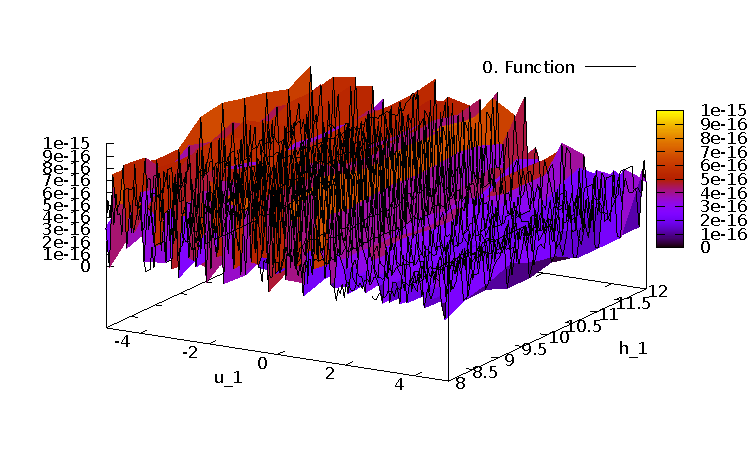
\includegraphics[scale=\zoomfactor]{{{2_points_def_luecke/x_y_0.0_10.0_0.0_10.0_0.0_10.0f0}}}
  % }
  %   \subfloat[Momentum error] {
  \begin{tikzpicture}
    \node at (0,0) {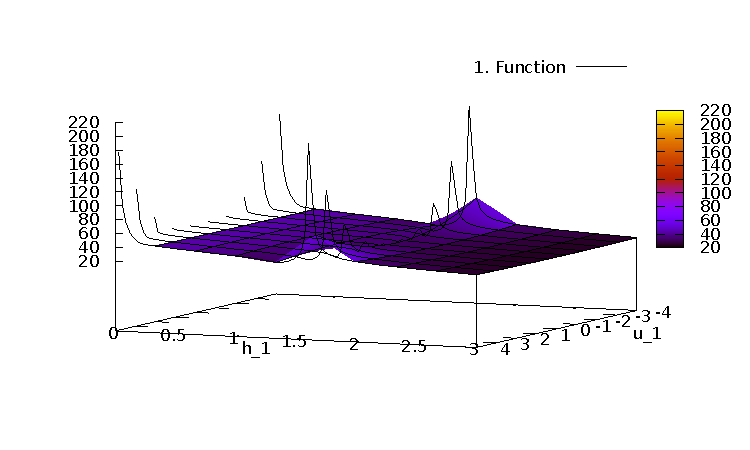
\includegraphics[scale=\zoomfactor]{{{2_points_def_luecke/x_y_0.0_10.0_0.0_10.0_0.0_10.0f1}}}};
    \fill[white] (.8,1.2) rectangle (1.75,1.5);
    \node[align=right, text width=3cm] at (.2,1.33) {\textsf{\tiny{Momentum error}}};
  \end{tikzpicture}
  % }
  \caption{Plotting the momentum error depending on $p_1$ for a wider range. All other points are $(10,0)$.}
  \label{fig:two-points-p1-wider-range}
\end{figure}

%%% Local Variables:
%%% TeX-master: "../results.tex"
%%% End:

%%% Local Variables:
%%% TeX-master: "../results.tex"
%%% End:
